\documentclass[12pt]{amsart}
\usepackage[T1]{fontenc}
\usepackage[utf8]{inputenc}
\usepackage{amsmath, amssymb, graphicx, hyperref, comment}
\usepackage{caption, subcaption}
\usepackage{adjustbox}
\usepackage[margin=1in,marginparwidth=0.75in]{geometry}
\usepackage{bm}

\hypersetup{
    colorlinks=true,
    linkcolor=blue,
    filecolor=black,      
    urlcolor=blue,
    citecolor=blue,
}

\newcommand\marginal[1]{\marginpar{\raggedright\parindent=0pt\tiny #1}}

\newtheorem{theorem}{Theorem}[section]
\newtheorem*{theorem*}{Theorem}
\newtheorem{lemma}[theorem]{Lemma}
\newtheorem*{lemma*}{Lemma}
\newtheorem{corollary}[theorem]{Corollary}
\newtheorem*{corollary*}{Corollary}
\newtheorem{prop}[theorem]{Proposition}
\newtheorem*{prop*}{Proposition}
\newtheorem{observation}[theorem]{Observation}
\newtheorem{construction}[theorem]{Construction}


\newtheorem{conjecture}[theorem]{Conjecture}
\newtheorem{question}[theorem]{Question}
\newtheorem{obs}[theorem]{Observation}
\newtheorem{claim}[theorem]{Claim}
\newtheorem{fact}[theorem]{Fact}

\theoremstyle{definition}
\newtheorem{definition}[theorem]{Definition}
\newtheorem*{definition*}{Definition}
\theoremstyle{remark}
\newtheorem{remark}[theorem]{Remark}

% theorems
\usepackage{thmtools}
\usepackage{thm-restate}

\usepackage{lipsum}


\DeclareMathOperator{\dist}{dist}
\DeclareMathOperator{\aut}{Aut}
\DeclareMathOperator{\gal}{Gal}
\DeclareMathOperator{\var}{\textbf{var}}
\DeclareMathOperator{\orb}{Orb}
\DeclareMathOperator{\ff}{Frac}
\DeclareMathOperator{\stab}{Stab}
\DeclareMathOperator{\inn}{Inn}
\DeclareMathOperator{\Ind}{Ind}
\DeclareMathOperator{\Res}{Res}
\DeclareMathOperator{\spn}{Span}
\DeclareMathOperator{\out}{Out}
\DeclareMathOperator{\ima}{Im}
\DeclareMathOperator{\dom}{Dom}
\DeclareMathOperator{\rk}{rk}
\DeclareMathOperator{\disc}{disc}
\DeclareMathOperator{\tors}{Tors}
\DeclareMathOperator{\Mor}{Mor}
\DeclareMathOperator{\End}{End}
\DeclareMathOperator{\Hom}{Hom}
\DeclareMathOperator{\Nat}{Nat}
\DeclareMathOperator{\spec}{Spec}
\DeclareMathOperator{\ann}{Ann}
\DeclareMathOperator{\ord}{ord}
\DeclareMathOperator{\conjc}{Conj}
\DeclareMathOperator{\Br}{Br}
\DeclareMathOperator{\Tr}{Tr}
\DeclareMathOperator{\Nm}{Nm}
\DeclareMathOperator{\Char}{char}
\DeclareMathOperator{\crossing}{cr}
\graphicspath{{Figures/}}

%────────────────────────────────────────────────────────────────────────────────────────────────────────────────────────────────────────────────────
%────────────────────────────────────────────────────────────────────────────────────────────────────────────────────────────────────────────────────

\begin{document}
\title{Basic template for mathematics reports} 

\author[Doe]{John Doe}
\address{Department of Mathematics\\
         Research Institution,
         City, State XXXXX
         Country} 
\email{jdoe@example.edu}
\date{\today}

\begin{abstract}
This is a latex template that demonstrates how you may type up a mathematics report in Latex. The reports in the summer REU at Indiana University can be found in \url{https://math.indiana.edu/undergraduate/reu-summer-research-program/past-reu/index.html}.

\end{abstract}

\maketitle

%────────────────────────────────────────────────────────────────────────────────────────────────────────────────────────────────────────────────────
%────────────────────────────────────────────────────────────────────────────────────────────────────────────────────────────────────────────────────

\textbf{There is an issue of not specifying what tends to infinity in some places. see crossing number inequalities and sum product theorems, say something like "when asymptotic parameter is not specified, take it to be..."}

\textbf{for all names add Dr or Mr or Professor or sum}

\textbf{less than less than epsilon notation}

\textbf{issue of "for any set A" in statements, but only as A gets sufficiently large}

\textbf{We presume the reader is familiar with basic ... such as ... }

\section{Introduction and Motivation} 

For any sets \(A,B\) and binary operation \(\cdot \) which acts on elements of \(A\) and \(B\), we define
\[
    A \cdot  B = \left\{ a \cdot  b : a \in A~,~ b \in B \right\} 
.\]

Observe the following 2 examples which motivate the study of the sum-product problem.

Let \(A\) be a finite set of numbers given by an arbitrary arithmetic sequence, and \(G\)
by an arbitrary geometric sequence. We will determine the size of the sets \(A + A, AA , G + G\), and \(GG\). 

\(A\) is of the form
\[
    A = \left\{ a , a + d , a+2d , \dots , a + (n-1)d \right\} 
\]
and \(G\) of the form
\[
    G = \left\{ b, br , br^{2}, \dots , br^{k - 1} \right\} 
.\]
Observe that
\begin{align*}
    \left\lvert A + A \right\rvert  & = \left\lvert \left\{ 2a, 2a + d, 2a + 2d ,\dots , 2a + 2(n-1)d \right\}  \right\rvert \\
    & = 2(n-1) + 1 \\
    & = 2 \left\lvert A \right\rvert - 1,
\end{align*}
and by the same argument,
\begin{align*}
    \left\lvert GG \right\rvert  & = \left\lvert \left\{ b^{2} , b^{2}r , \dots , b^{2}r^{2(k-1)} \right\} \right\rvert  \\
    & =2 \left\lvert G \right\rvert -1.
\end{align*}
We have
\begin{align*}
    \left\lvert G + G \right\rvert & = \left\lvert \left\{ g_1 + g_2 : g_1,g_2 \in G \right\} \right\rvert  \\
    & = \left\lvert \left\{ b(r^{i} + r^{j}): i,j \in \left\{ 0, \dots , k-1 \right\}  \right\} \right\rvert \\
    & = \left\lvert \left\{r^{i} + r^{j}: i,j \in \left\{ 0, \dots , k-1 \right\}  \right\} \right\rvert.
\end{align*}
For \(i \neq j\), \(r^{i} + r^{j}\) represents a number in base \(r\). By the uniqueness of representations
in different bases (see appendix) \textbf{PUT IT IN APPENDIX}, we can conclude that there must be at least \(k^{2}- k\) many numbers in this set, that is
\[
    \left\lvert G + G \right\rvert = \left\lvert \left\{ r^{i} + r^{j} : i,j \in \left\{ 0 , \dots , k-1 \right\}   \right\}  \right\rvert \geq k^{2}- k = \left\lvert G \right\rvert ^{2} - \left\lvert G \right\rvert 
.\]

\textbf{I NEED TO FINISH THIS EXAMPLE}
\textbf{fix G sum set}

Observing the trivial bound \(\left\lvert S \cdot S \right\rvert \leq \left\lvert S \right\rvert ^{2}\) for any set \(S\) and any
operation \(\cdot \), it is clear that both \(AA\) and \(G +G\) are almost as large as they can be.

The main questions is: ``does there exist a set for which both the sum and product sets are small?''
The sum-product conjecture states that such a set does not exist. Another good question is: ``what
determines whether the sum set is large or the product set is large?'' A separate
conjecture tries to partially answer this question by stating that the sum set is large
when the set itself is convex.

\textbf{ABOVE PARAGRAPH CONVEX PRODUCT SET ARGUMENT}

The rest of the report will proceed in the following way : \textbf{finish this}

\section{Preliminaries}

For any natural number \(n\), define
\[
    [n] = \left\{ 1, 2 , \dots , n \right\} 
.\]

For any functions \(f,g: \mathbb{N}  \to \mathbb{R} \), write
\[
    f(x) \gg g(x) 
\]
if
\[
    \exists x_0 \in \mathbb{N} ~~\text{s.t.}~~ x > x_0 \implies \left\lvert f(x) \right\rvert \geq c \left\lvert g(x) \right\rvert  
,\]
write
\[
    f(x) \ll g(x) 
\]
if
\[
    \exists x_0 \in \mathbb{N} ~~\text{s.t.}~~ x > x_0 \implies \left\lvert f(x) \right\rvert \leq c \left\lvert g(x) \right\rvert 
,\]
and write
\[
    f(x) \asymp g(x)
\]
if
\[
    f(x) \ll g(x) ~ ~ \text{and} ~ ~ f(x) \gg g(x)
.\]

For any sets \(A,B\) and any binary operation \(\cdot \) acting on elements of \(A\) and \(B\), define the representation function
\(r_{A \cdot B} : A \cdot B \to \mathbb{N} \) by
\[
    r_{A \cdot B} (x) = \left\lvert \left\{ (a,b)\in  A \times B : x = a \cdot b \right\}  \right\rvert
.\]

For any sets \(A,B\), define the Additive Energy \(E(A,B)\) and Multiplicative Energy \(M(A,B)\) by
\[
    E(A,B) = \left\lvert \left\{ (a_1,a_2,b_1,b_2) \in A^{2} \times B^{2} : a_1 + b_1 = a_2 + b_2 \right\}  \right\rvert 
\]
and
\[
    M(A,B) = \left\lvert \left\{ (a_1,a_2,b_1,b_2)\in  A^{2} \times B^{2} : a_1b_1 = a_2b_2 \right\}  \right\rvert
.\]

Observe that
\[
    E(A,B) = \sum _{x \in A + B} r_{A+B} (x)^{2}
\]
and
\[
    M(A,B) = \sum _{x \in AB} r_{AB} (x)^{2} 
.\]

A 4-tuple \((a_1,a_2,b_1,b_2)\in A^{2} \times B^{2}\) is a solution to
\[
    a_1 + b_1 = a_2 + b_2
\]
if and only if it is a solution to
\[
    a_1-b_2 = a_2-b_1
,\]
and therefore
\[
    E(A,B) = \sum _{x \in A + B} r_{A+B} (x)^{2} = \sum _{x \in A - B} r_{A-B} (x)^{2}
.\]

%────────────────────────────────────────────────────────────────────────────────────────────────────────────────────────────────────────────────────
%────────────────────────────────────────────────────────────────────────────────────────────────────────────────────────────────────────────────────

\textbf{FINISH BELOW}
Any 4-tuple \((a_1,a_2,b_1,b_2) \in A^{2} \times B^{2}\) with nonzero entries is a solution to
\[
    a_1b_1 = a_2b_2
\]
if and only if it is a solution to
\[
    \frac{a_1}{b_2} = \frac{a_2}{b_1} 
,\]
and therefore

%────────────────────────────────────────────────────────────────────────────────────────────────────────────────────────────────────────────────────
%────────────────────────────────────────────────────────────────────────────────────────────────────────────────────────────────────────────────────

By the Cauchy-Schwarz Inequality
\[
    \left\lvert A \right\rvert \left\lvert B \right\rvert = \sum _{x \in A + B} r_{A + B} (x) \leq \left\lvert A + B \right\rvert ^{\frac{1}{2} } E(A,B)^{\frac{1}{2} }
,\]
and
\[
    \left\lvert A \right\rvert \left\lvert B \right\rvert = \sum _{x \in AB} r_{AB} (x) \leq \left\lvert AB \right\rvert ^{\frac{1}{2} }M(A,B)^{\frac{1}{2} }
.\]
Similar inequalities can be derived for \(\left\lvert A-B \right\rvert \) and \(\left\lvert \frac{A}{B}  \right\rvert \).

%────────────────────────────────────────────────────────────────────────────────────────────────────────────────────────────────────────────────────
%────────────────────────────────────────────────────────────────────────────────────────────────────────────────────────────────────────────────────


\textbf{CONVEXITY}
Let \(I \subset \mathbb{R} \) be an interval. 
    A function \(f: I \to \mathbb{R} \) is convex if for
    any 2 points \(x_1,x_2 \in I\), and any \(\lambda \in [0,1]\),
    \[
        f((x_1-x_2)\lambda + x_2) \leq \left( f(x_1)-f(x_2) \right) \lambda + f(x_2)
    .\]

    A finite set \(A \subset \mathbb{R}\) is convex if there is a function \(f: [1, \left\lvert A \right\rvert ] \to \mathbb{R} \)
such that
\[
    A = \left\{ f(i) : i \in \left\{ 1, \dots , \left\lvert A \right\rvert  \right\}  \right\} 
.\]

%────────────────────────────────────────────────────────────────────────────────────────────────────────────────────────────────────────────────────
%────────────────────────────────────────────────────────────────────────────────────────────────────────────────────────────────────────────────────


\section{ \textbf{IDK what to call this}}
The idea that there does not exist a set with a small sum and product set is
stated precisely as
\begin{conjecture}[Sum-Product Conjecture]
For every sufficiently large finite set \(A \subset \mathbb{R} \),
\[
    \max \left( \left\lvert A+A \right\rvert ~,~ \left\lvert A \cdot A \right\rvert  \right) \gg_{\epsilon}  \left\lvert A \right\rvert^{2-\epsilon}
\]
\end{conjecture}

The idea that 

\begin{conjecture}
    For every sufficiently large, finite, and convex set \(A\),
    \[
        \left\lvert A+A \right\rvert \gg_{\epsilon}  \left\lvert A \right\rvert ^{2-\epsilon}
    \]
\end{conjecture}

To date, the best results for both of these conjectures are proven in \textbf{ref}.

\textbf{proven in this report?}

they are
\begin{theorem}
    For every sufficiently large finite set \(A \subset \mathbb{R} \),
    \[
        \max \left( \left\lvert A+A \right\rvert ~,~ \left\lvert A \cdot A \right\rvert  \right) \gg_{\epsilon}   \left\lvert A \right\rvert^{\frac{4}{3} + \frac{2}{1167} - \epsilon}
    \]
\end{theorem}

and

\begin{theorem}
    For every sufficiently large, finite, and convex set \(A\),
    \[
        \left\lvert A+A \right\rvert \gg_{\epsilon}  \left\lvert A \right\rvert ^{\frac{30}{19} - \epsilon }
    \]
\end{theorem}

\textbf{if not, best results in this are ... , others are only slight improvements}

A final result I'd like to mention, which I found interesting, is a result by Olmezov
proven in \textbf{ref}

\begin{theorem}
    Let \(n \geq 1\). Let \(f: [1,n]\to \mathbb{R} \) be a convex function satisfying
    \[
    f^{\prime}(x)>0, \quad f^{\prime \prime}(x)>0, \quad f^{\prime \prime \prime}(x)<0, \quad f^{(I V)}(x) \leq 0,
    \]
    and let \(A=\{f(i): i=1, \ldots, n\}\). Then
    \[
        \left\lvert A \pm A \right\rvert \gg_{\epsilon} \left\lvert A \right\rvert ^{\frac{5}{3} - \epsilon}
    .\]
\end{theorem}

I will not discuss this result further in this paper.

\section{Graphs and the Crossing Number Inequality}

\textbf{Make a note about how this is the dumbed down version (no topology)}

A very useful tool in proving sum-product theorems is the Szemeredi-Trotter theorem. The
easiest proof of this theorem is as a corollary of the Crossing Number Inequality, which gives
an estimate on how close a graph is to being planar. The purpose of this section
is to provide a brief introduction to graphs and prove the Crossing Number Inequality.

\textbf{define connected}
\textbf{Tao's article reread to see what I missed}

Abstractly, a graph \(G\) is a pair \(G = (V,E)\) where each \(e \in E\) is of the form \(e \subset V\) with \(\left\lvert e \right\rvert = 2\).
The call the set \(V\) the vertices, and the set \(E\) the edges. A drawing of a graph
is a depiction of a graph with vertices as points in the plane and edges as curves between the
vertices they consist of. For example:

\begin{figure}[h]
    \centering
    \subfloat{{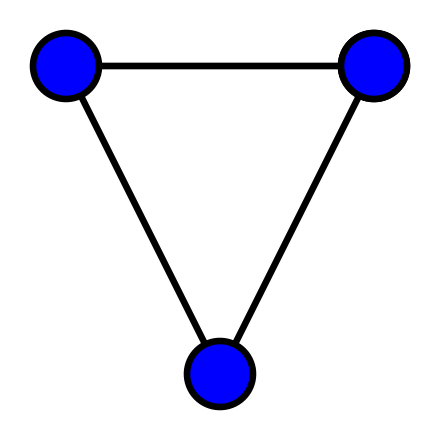
\includegraphics[width=4cm]{3graph.png} }}
    \qquad
    \subfloat{{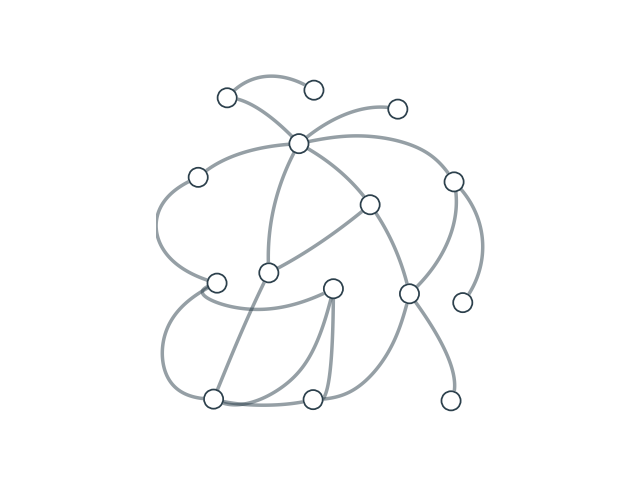
\includegraphics[width=6cm]{cgraph.png} }}
    \caption{Drawings of Graphs}
\end{figure}

There are infinitely many ways to draw any given graph. A crossing in a drawing
of a graph is an intersection between 2 curves which represent edges. The 
crossing number of a graph is the minimum number of crossings
over all drawings of the graph \(G\). Denote this by
\(\crossing(G)\). A graph \(G\) is called planar if its crossing number is 0.

A precise statement of the Crossing Number Inequality is

\begin{theorem}\label{thm:crossing-number-inequality}
    If \(G = (V,E)\) is a sufficiently large graph, with \(\left\lvert E \right\rvert \geq 4 \left\lvert V \right\rvert \),
    then
    \[
        \crossing\left( G \right) \gg \frac{\left\lvert E \right\rvert ^{3} }{\left\lvert V \right\rvert ^{2}}  
    .\]
\end{theorem}

For a drawing of a planar graph, we call any region of the plane which is bounded by edges a face. We also call
the unbounded region of the plane a face. Here is an example of a drawing of a planar
graph with labelled faces:

\begin{figure}[h]
    \centering
    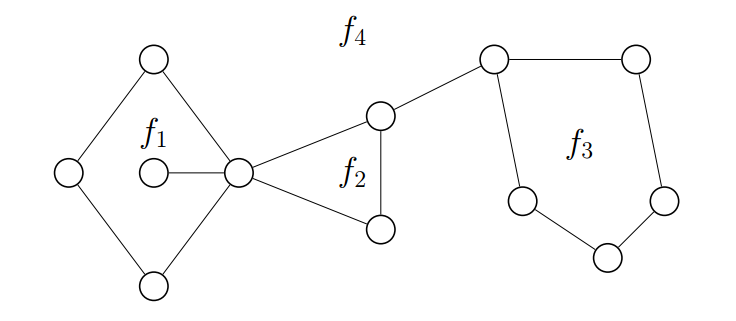
\includegraphics[width=0.6\textwidth]{faceimage.png}
    \caption{Drawing of Planar Graph with Labeled Faces \(f_{i} \)}
\end{figure}

Observe that any non-planar graph \(G = (V,E)\) can be turned into a planar graph by removing at most
\(\crossing\left( G \right) \) edges from \(E\). Therefore, an upper bound on the number of edges of a
planar graph can be used to find a lower bound on the crossing number of a non-planar graph.
An obvious tool to use for a statement about planar graphs is

\begin{theorem}[Euler's Formula for Planar Graphs]\label{thm:euler-formula-graphs}
Let \(G = (V,E)\) be a connected planar graph, with \(\left\lvert V \right\rvert \geq 1\), and consider some drawing with 0 crossings.
Let \(F\) be the set of all faces of this drawing.
\[
    \left\lvert V \right\rvert - \left\lvert E \right\rvert + \left\lvert F \right\rvert = 2
.\]
\end{theorem}

\begin{proof}
We may construct our drawing of \(G\) by first drawing a vertex, and then doing combination of the following steps: 

\textbf{FINISH PROOF}
\end{proof}


\textbf{below paragraph is ugly}
The dependence on \(\left\lvert F \right\rvert \) in Euler's formula can be removed by bounding
it in terms of \(\left\lvert E \right\rvert \). This can be done by double counting the face-edge
incidences. Let an edge be incident to a face if the edge is one of the bounding
edges which defines the face. Define \(\chi : F \times E \to \left\{ 0,1 \right\} \) by
\(\chi(f,e) = 1\) if \(f\) and \(e\) are incident, and \(\chi(f,e) = 0\) otherwise.
The total number of face edge incidences is
\[
    I = \sum_{f\in F} \sum _{e \in E} \chi(f,e)
.\]
We may assume \(E \geq 3\). It follows that every face is incident to at least 3 edges,
so
\[
    I \geq \sum _{f \in F} 3 = 3 \left\lvert F \right\rvert 
.\]
Every edge is incident to at most 2 faces, so
\[
    I \leq \sum _{e \in E} 2 = 2 \left\lvert E \right\rvert 
.\]
It follows that
\[
    3 \left\lvert F \right\rvert \leq 2 \left\lvert E \right\rvert 
\]
or
\[
    \left\lvert F \right\rvert \leq \frac{2}{3} \left\lvert E \right\rvert 
.\]
Applying this to Euler's formula,
\[
    \left\lvert V \right\rvert - \left\lvert E \right\rvert + \frac{2}{3} \left\lvert E \right\rvert \geq 2
\]
or
\[
    \left\lvert E \right\rvert \leq 3 \left\lvert V \right\rvert -6
.\]
Now suppose that \(G = (V,E)\) is non-planar. As mentioned before, \(G\) may be turned planar
\textbf{I NEED BETTER LOGIC FOR WHY I CAN REMOVE CRG AND MAKE IT PLANAR}


Therefore, if \(\left\lvert E \right\rvert \geq 3 \left\lvert V \right\rvert \), then \(\crossing\left( G \right) \geq \left\lvert E \right\rvert  - 3 \left\lvert V \right\rvert \).
To further improve this inequality, apply the probabilistic method to the deletion of vertices of \(G\).

Let each \(v \in V\) be
removed with a probability \(1-p~,~  p \in (0,1)\). Let the remaining set of vertices be \(V'\). An edge is
removed whenever either of the corresponding vertices are removed. Let the remaining set of edges be \(E'\). The remaining graph is then
\(G' = (V',E')\). We have
\[
    \crossing\left( G' \right) \geq \left\lvert E' \right\rvert - 3 \left\lvert V' \right\rvert 
,\]
and so
\[
    \mathbb{E} \left( \crossing\left( G' \right)  \right) \geq \mathbb{E} \left( \left\lvert E' \right\rvert - 3 \left\lvert V' \right\rvert  \right) 
,\]
or, by the linearity of the expected value,
\[
    \mathbb{E} \left( \crossing\left( G' \right)  \right) \geq \mathbb{E} \left( \left\lvert E' \right\rvert  \right) - 3 \mathbb{E} \left( \left\lvert V' \right\rvert  \right)    
.\]
Each \(v \in V\) is removed with probability \(1-p\), so
\[
    \mathbb{E} \left( \left\lvert V' \right\rvert  \right) = p \left\lvert V \right\rvert 
.\]
Each edge remains only when both corresponding vertices remain. Each vertex remains
independently with a probability \(p\), so 
\[
    \mathbb{E} \left( \left\lvert E' \right\rvert  \right) = p^{2}\left\lvert E \right\rvert 
.\]
Considering a drawing of \(G\) with the minimum number of crossings. Each crossing remains
only if both corresponding edges remain. Each edge remains independently with a probability
\(p^{2}\), so the expected value of the number of crossings remaining in the drawing is \(p^{4} \crossing\left( G \right) \).
There is no guarantee that this drawing is optimal to minimize the crossings of \(G'\), but we may conclude that
\[
    \mathbb{E} \left( \crossing\left( G' \right)  \right) \leq p ^{4} \crossing\left( G \right)
,\]
and therefore that
\[
    p^{4} \crossing\left( G \right) \geq \mathbb{E} \left( \crossing\left( G \right)  \right) \geq p^{2} \left\lvert E \right\rvert - 3 p \left\lvert V \right\rvert 
\]
for any \(p \in (0,1)\). Assuming \(\left\lvert E \right\rvert \geq 4\left\lvert V \right\rvert \), and taking \(p = \frac{4\left\lvert V \right\rvert }{\left\lvert E \right\rvert }\),
\[
    \crossing\left( G \right) \geq \frac{\left\lvert E \right\rvert }{\left( \frac{4 \left\lvert V \right\rvert }{\left\lvert E \right\rvert }   \right)^{2} } - \frac{3 \left\lvert V \right\rvert }{\left( \frac{4 \left\lvert V \right\rvert }{\left\lvert E \right\rvert }  \right) ^{3} } = \frac{1}{16} \left( \frac{\left\lvert E \right\rvert ^{3} }{\left\lvert V \right\rvert ^{2}} - \frac{3 \left\lvert E \right\rvert ^{3} }{4 \left\lvert V \right\rvert ^{2}}  \right) \gg \frac{\left\lvert E \right\rvert ^{3} }{\left\lvert V \right\rvert ^{2}}
.\]

\section{The Szemeredi-Trotter Theorem}

A precise statement of the Szemeredi-Trotter Theorem is

\textbf{I think there is a better way to write the set of curves below that is less restrictive on their domain}

\begin{theorem}[Szemeredi-Trotter Theorem]
Let \(P \subset \mathbb{R} ^{2}\) be a finite set of points. Let \(\mathcal{L} \) be a finite set of curves in \(\mathbb{R} ^{2}\). 

More precisely,
every \(l \in \mathcal{L} \) is of the form \(l = \left\{ (x(t),y(t)) : t\in \mathbb{R}  \right\} \) for some \(x,y \in C^{0}(\mathbb{R} )\). 

Let \(\chi : P \times \mathcal{L}  \to \left\{ 0,1 \right\} \) be the incidence function
between a point and a line, so
\[
\chi(p,l) = 
\begin{cases}
1 ~ ~ \text{if} ~ ~ p\in l\\
0 ~ ~ \text{otherwise} 
\end{cases}
\]

If any two \( l \in \mathcal{L} \) intersect in at most one point,
then the total number of point-line incidences,
\[
    I(P, \mathcal{L} ) = \sum _{(p,l)\in P \times \mathcal{L} } \chi(p,l)
\]
satisfies
\[
    I(P,\mathcal{L} ) \ll  \left\lvert P \right\rvert^{\frac{2}{3} } \left\lvert \mathcal{L}  \right\rvert ^{\frac{2}{3} } + \left\lvert P \right\rvert + \left\lvert \mathcal{L}  \right\rvert 
.\]
\end{theorem}

\textbf{First proven in ...}

\textbf{I need to prove that the crossing number inequality can be used}

\textbf{Proof}

\textbf{revise below dialogue}

A particular case of the Szemeredi-Trotter theorem is when all the curves in \(\mathcal{L} \) are lines.
Heuristically, the Szemeredi-Trotter theorem is useful in the study of Sum-Product problems
because equations of lines are given by addition and multiplication. You can construct a system of
lines and points whose incidences relate to the sum or product set you are studying, and apply the Szemeredi-Trotter
theorem to bound these incidences.

Recalling the property of convexity, \textbf{... finish this dialogue}.

\begin{theorem}
    For sufficiently large sets \(A \subset \mathbb{R} \),
    \[
        \max \left( \left\lvert A+A \right\rvert, \left\lvert A\cdot A \right\rvert  \right) \gg \left\lvert A \right\rvert ^{\frac{5}{4} }
    .\]
\end{theorem}

\begin{proof}
Take \(P = \left( A + A \right) \times \left( A \cdot A \right) \). 

For any \(a,b \in A\), let \(\ell _{a,b} : \mathbb{R} \to \mathbb{R} \) be defined by
\(\ell _{a,b} (x) = (x-a)\cdot b\). Let \(L_{a,b} = \left\{ (x, \ell _{a,b} (x)) : x \in \mathbb{R}  \right\} \)
be the graph of \(\ell _{a,b} \).

Take \(\mathcal{L} = \left\{ L_{a,b} : a,b \in A \right\} \). There are \(\left\lvert A \right\rvert \) many numbers in
\(A + A\) of the form \(x + a\) where \(x \in A\). For all of these numbers, \(\ell _{a,b} (x + a) = xb \in A\cdot A\).

We have shown that for each choice of \(a,b \in A\), there are \(\left\lvert A \right\rvert \) many numbers
\(z \in A+A\) such that \(\ell _{a,b} (z) \in A\cdot A\), or that there are \(\left\lvert A \right\rvert \) many
incidences between \(P\) and \(L_{a,b} \). It follows that there are \(\left\lvert A \right\rvert ^{3} \) total incidences
between \(\mathcal{L} \) and \(P\). Because \(\mathcal{L} \) is a set of lines, the Szemeredi-Trotter theorem holds.

\[
    \left\lvert A \right\rvert ^{3} \ll \left\lvert A + A \right\rvert ^{\frac{2}{3} } \left\lvert A \cdot A \right\rvert ^{\frac{2}{3} } \left\lvert A \right\rvert ^{\frac{4}{3} } + \left\lvert A + A \right\rvert \left\lvert A \cdot A \right\rvert + \left\lvert A \right\rvert ^{2}
\]
or
\[
    \left\lvert A \right\rvert ^{3} \ll \max \left( \left\lvert A + A \right\rvert ^{\frac{2}{3} } \left\lvert A \cdot A \right\rvert ^{\frac{2}{3} } \left\lvert A \right\rvert ^{\frac{4}{3} } , \left\lvert A + A \right\rvert \left\lvert A \cdot A \right\rvert , \left\lvert A \right\rvert ^{2} \right) 
.\]

Applying trivial inequalities,
\[
    \left\lvert A \right\rvert ^{2} \leq \left\lvert A+A \right\rvert \left\lvert A \cdot A \right\rvert \leq \left\lvert A+A \right\rvert \left\lvert A \cdot A \right\rvert \left( \frac{\left\lvert A \right\rvert ^{\frac{4}{3} }}{\left\lvert A+A \right\rvert ^{\frac{1}{3} }\left\lvert A \cdot A \right\rvert ^{\frac{1}{3} }}  \right) 
,\]
so
\begin{align*}
    \left\lvert A \right\rvert ^{3} \ll \left\lvert A+A \right\rvert ^{\frac{2}{3} }\left\lvert A \cdot A \right\rvert ^{\frac{2}{3} } \left\lvert A \right\rvert ^{\frac{4}{3} } & \implies \max \left( \left\lvert A + A \right\rvert , \left\lvert A \cdot A \right\rvert  \right) ^{\frac{4}{3} } \gg \left\lvert A \right\rvert ^{\frac{5}{3} } \\
    & \implies \max \left( \left\lvert A + A \right\rvert , \left\lvert A \cdot A \right\rvert  \right) \gg \left\lvert A \right\rvert ^{\frac{5}{4} }.
\end{align*}

\end{proof}

\begin{theorem}\label{thm:elekes-non-general}
For sufficiently large sets \(A \subset \mathbb{R} \) which are finite and convex,
\[
    \left\lvert A+A \right\rvert \gg \left\lvert A \right\rvert ^{\frac{3}{2} }
.\]
\end{theorem}

More generally,

\begin{theorem}

    For sufficiently large sets \(A \subset \mathbb{R} \), which are finite and convex,
\[
    \left\lvert A + B \right\rvert \gg \left\lvert A \right\rvert ^{\frac{3}{2} }
\]
for any set \(B \subset \mathbb{R} \) with \(\left\lvert A \right\rvert = \left\lvert B \right\rvert \).
\end{theorem}

\begin{proof}
ok
\end{proof}

Theorem \ref{thm:elekes-non-general} follows immediately from this.

We also have results like

\begin{theorem}

    Let \(A \subset \mathbb{R} \) be a sufficiently large convex and finite set, then for every 
    finite set \(B \subset \mathbb{R} \) we have

    \[
        \left\lvert \left\{ x \in A-B : \delta_{A,B} (x) \geq \tau \right\}  \right\rvert \ll \frac{\left\lvert A \right\rvert \left\lvert B \right\rvert }{\tau^{3} }
    .\]
\end{theorem}

\textbf{any more results here?}

\section{Additive Energy Estimates}

\textbf{is this section worthy?}

\textbf{why additive energy?}


%────────────────────────────────────────────────────────────────────────────────────────────────────────────────────────────────────────────────────
%────────────────────────────────────────────────────────────────────────────────────────────────────────────────────────────────────────────────────

\subsection*{Acknowledgements} % Unnumbered subsection to include acknowledgements (advisor, grants, etc.) An example acknowledgement is included for reference. 
This report is based on work supported by NSF grant DMS-2051032, which we gratefully acknowledge. I would also like to express my thanks to the Mathematics department of Indiana University for hosting the program, my mentor XXX and....


%% TIP: Only entries which you actually cite with \cite somewhere else in the .tex will appear.
\bibliographystyle{amsalpha}
\bibliography{bibliography} % the file "bibliography.bib" will be needed

\section*{Appendix}

It can be useful to include additional information, long calculations that disrupt the main flow of the proof, etc. in an appendix section (usually unnumbered).

\end{document}